\documentclass{standalone}
\usepackage{tikz}


\begin{document}
    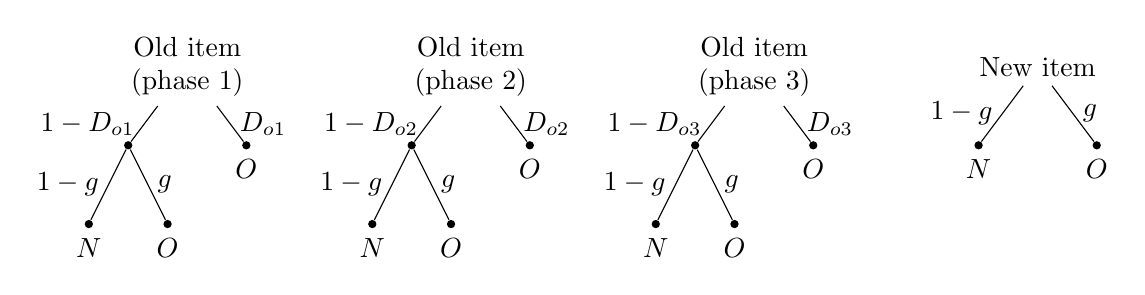
\begin{tikzpicture}[x=1.2cm, y=1.5cm]
        \tikzset{
            level 1/.style={level distance=1cm, sibling distance=1.5cm},
            level 2/.style={level distance=1cm, sibling distance=1cm},
            bag/.style={text width=5em, text centered},
            end/.style={circle, minimum width=3pt, fill, inner sep=0pt}
        }

        % Tree 1 - Old item
        \node[bag] (old1) at (0,0) {Old item\\(phase 1)}
            child {
                node[end] {}        
                    child {
                        node[end, label=below: {$N$}] {}
                        edge from parent node[left] {$1-g$}
                    }
                    child {
                        node[end, label=below: {$O$}] {}
                        edge from parent node[right] {$g$}
                    }
                    edge from parent node[left] {$1-D_{o1}$}
            }
            child {
                node[end, label=below: {$O$}] {} 
                edge from parent node[right] {$D_{o1}$}     
            };

        % Tree 2 - Old item
        \node[bag] (old2) at (3,0) {Old item\\(phase 2)}
            child {
                node[end] {}        
                    child {
                        node[end, label=below: {$N$}] {}
                        edge from parent node[left] {$1-g$}
                    }
                    child {
                        node[end, label=below: {$O$}] {}
                        edge from parent node[right] {$g$}
                    }
                    edge from parent node[left] {$1-D_{o2}$}
            }
            child {
                node[end, label=below: {$O$}] {} 
                edge from parent node[right] {$D_{o2}$}     
            };

        % Tree 3 - Old item
        \node[bag] (old3) at (6,0) {Old item\\(phase 3)}
            child {
                node[end] {}        
                    child {
                        node[end, label=below: {$N$}] {}
                        edge from parent node[left] {$1-g$}
                    }
                    child {
                        node[end, label=below: {$O$}] {}
                        edge from parent node[right] {$g$}
                    }
                    edge from parent node[left] {$1-D_{o3}$}
            }
            child {
                node[end, label=below: {$O$}] {} 
                edge from parent node[right] {$D_{o3}$}     
            };

        % Tree 4 - New item
        \node[bag] (new1) at (9,0) {New item}
            child {
                node[end, label=below: {$N$}] {} 
                edge from parent node[left] {$1-g$}
            }
            child {
                node[end, label=below: {$O$}] {} 
                edge from parent node[right] {$g$}     
            };
    \end{tikzpicture}

\end{document}